\documentclass[journal]{IEEEtran}
\usepackage[utf8]{inputenc}
\usepackage[T1]{fontenc}
\usepackage{amsmath,amssymb}
\usepackage{graphicx}
\usepackage{booktabs}
\usepackage{multirow}
\usepackage{array}
\usepackage{xcolor}
\usepackage{cite}
\usepackage{url}
\usepackage{tikz}
\usetikzlibrary{positioning,fit,arrows.meta}
\usepackage[hidelinks]{hyperref}
\graphicspath{{figures/}}
% Items the authors must confirm before submission are printed in red.
\newcommand{\tbc}[1]{\textcolor{red}{[TO CONFIRM: #1]}}
\newcommand{\code}[1]{\texttt{\small #1}}
\newcolumntype{L}[1]{>{\raggedright\arraybackslash}p{#1}}

\begin{document}

\title{HAIDS-PoA: A Labeled Node-Telemetry Intrusion Dataset for Ethereum Proof-of-Authority Networks and a Session-Aware Benchmark}

\author{Mariem~Ben~Abdallah, Zaineb~Sboui, and Eya~Hadj~Abdallah%
\thanks{The authors are with the Department of Computer Engineering \& Applied Mathematics, National Engineering School of Sfax (ENIS), Sfax, Tunisia.}%
\thanks{Dataset, code and all result files: \tbc{public repository URL}.}}

\maketitle

\begin{abstract}
Publicly available intrusion detection datasets describe conventional IP traffic and do not capture the peer-to-peer, mempool, and remote procedure call (RPC) behaviour of blockchain nodes. This paper introduces HAIDS-PoA, a labeled multiclass dataset of node-state telemetry collected on a seven-node Ethereum Clique Proof-of-Authority testnet deployed on three physical machines. The dataset contains 29{,}472 records sampled at a nominal two-second interval over 18.6~hours, organised in 35~recording sessions on six days, and covers benign operation and four attacks: Eclipse, Sybil, Transaction Flooding, and RPC Abuse. Because the recording sessions are preserved, HAIDS-PoA supports an evaluation that most intrusion detection benchmarks cannot perform: testing on recording days that were never seen during training. Using a leakage-free pipeline and six models, we report four findings. First, the evaluation protocol dominates the reported score: four classifiers reach a macro-F1 of 1.00 under a random split or a within-session chronological split, and 0.80--0.87 on unseen days. Second, the loss is caused by operating-system telemetry that identifies the recording session rather than the attack: node-level telemetry alone reaches 0.95 on unseen days, operating-system telemetry alone 0.66, and removing the operating-system network counters raises the full model from 0.83 to 0.98. Third, deciding \emph{whether} an attack is in progress transfers across days (F1 0.99) while deciding \emph{which} attack does not. Fourth, a supervised detector misses attack types absent from its training data (recall 0.4--49\%), whereas an autoencoder trained on benign data alone detects 88--100\% of them. We also provide a feature-layer and detection-pipeline ablation, complete hyperparameters, and measured training and inference costs.
\end{abstract}

\begin{IEEEkeywords}
Blockchain security, Proof-of-Authority, Ethereum, Clique, intrusion detection, labeled dataset, anomaly detection, evaluation protocol, data leakage, Eclipse attack, Sybil attack, transaction flooding, RPC abuse.
\end{IEEEkeywords}

\section{Introduction}
\IEEEPARstart{B}{lockchain} technology is now used as infrastructure for enterprise systems, supply-chain traceability, healthcare record management, and inter-organisational data sharing~\cite{zheng2018}. In these settings performance and governance are often prioritised over open participation, and permissioned architectures have become a practical alternative to public Proof-of-Work networks~\cite{wood2014}. Proof-of-Authority (PoA) consensus, in which a predefined set of validators seals blocks, is a common choice for consortium deployments~\cite{deangelis2018}; within the Ethereum ecosystem, the Clique protocol~\cite{eip225} is widely adopted because of its simplicity and its compatibility with Go-Ethereum (Geth).

PoA nodes remain exposed to network-layer threats. Ethereum nodes communicate through the DevP2P peer-to-peer protocol and expose a JSON-RPC interface. Eclipse attacks~\cite{heilman2015,marcus2018} surround a target with adversarial peers and isolate it from honest participants; Sybil attacks~\cite{douceur2002} introduce many malicious identities to manipulate the peer table; transaction flooding~\cite{baqer2016} overwhelms the mempool; and RPC abuse exhausts node resources through high-frequency or computationally expensive requests.

Detecting these attacks with machine learning is hindered by the lack of suitable data. Most intrusion detection studies rely on datasets such as NSL-KDD~\cite{tavallaee2009} and CICIDS-2017~\cite{sharafaldin2018}, which describe IP-layer traffic and do not represent peer churn, mempool pressure, or RPC responsiveness~\cite{saad2020}. Models trained on them cannot be assumed to generalise to Ethereum consortium environments~\cite{sommer2010}. To the best of our knowledge, no public labeled dataset targets multiclass intrusion detection in Ethereum Clique PoA networks using operational node telemetry.

A second, less visible problem concerns how such datasets are evaluated. Telemetry sampled every few seconds is strongly autocorrelated, and attacks are usually recorded in dedicated sessions. A random train/test split therefore places near-duplicate neighbours of every test record in the training set, and even a chronological split inside a session lets a model learn properties of the session (the machine state on that day) instead of properties of the attack. Both effects are known sources of over-optimistic results in security machine learning~\cite{arp2022,kapoor2023,pendlebury2019}, but a dataset can only expose them if its recording sessions are preserved and the same behaviour was recorded on more than one occasion.

This paper introduces HAIDS-PoA, a labeled dataset collected on a seven-node Ethereum Clique testbed distributed over three physical machines, together with a session-aware benchmark.

\subsection{What new scientific insights does HAIDS-PoA enable?}
HAIDS-PoA keeps the timestamp and session of every record, and benign operation, Eclipse, Flooding and RPC Abuse were each recorded on at least two different days. This makes it possible to measure, rather than assume, how a blockchain intrusion detector behaves on a day it has never seen. With it we establish four findings.

\begin{enumerate}
\item \textbf{The evaluation protocol decides the score.} Logistic regression, Random Forest, XGBoost and LightGBM all reach a macro-F1 of 1.00 under a random row split and under a within-session chronological split. Tested on unseen recording days, the same models reach 0.80--0.87 (Section~\ref{sec:res-protocol}).
\item \textbf{Node telemetry generalises; operating-system telemetry does not.} On unseen days, features taken from the node itself (peer table, mempool, gas, RPC latency) reach a macro-F1 of 0.95, whereas CPU, memory and operating-system network counters reach 0.66. Removing the operating-system network counters alone raises the full model from 0.83 to 0.98, because a quantity such as the number of open connections identifies the recording day rather than the attack (Section~\ref{sec:res-ablation}).
\item \textbf{Detection transfers across days; attack typing does not.} A binary detector keeps an F1 of 0.99 on unseen days, and a two-stage pipeline (anomaly alarm, then attack typing) outperforms a single five-class classifier, 0.89 against 0.83 (Section~\ref{sec:res-pipeline}).
\item \textbf{Unseen attack types require benign-only models.} A supervised detector that never saw a given attack detects 0.4--49\% of its records, whereas an autoencoder trained on benign data alone detects 88--100\%. The ranking produced by benign-only detectors is stable across days (ROC-AUC $\geq 0.985$), but a fixed alarm threshold is not (Section~\ref{sec:res-anomaly}).
\end{enumerate}

\subsection{Contributions}
\begin{enumerate}
\item A seven-node Ethereum Clique PoA testbed on three physical machines, with a telemetry collector that polls the victim node across the peer-to-peer, chain, RPC and host layers.
\item The HAIDS-PoA dataset: 29{,}472 labeled records in five classes, 16 raw metrics and 7 collector-derived quantities per record, released with timestamps and session boundaries (35 sessions, six days).
\item A leakage-free preprocessing pipeline in which every derived feature is causal, computed inside one session, and independent of the label, and in which chain-instance identifiers are excluded.
\item Three evaluation protocols of increasing strictness, including a cross-day protocol, and a benchmark of six models with five random seeds.
\item A feature-layer ablation, a detection-pipeline ablation, and an unseen-attack experiment.
\item Complete hyperparameters and measured training and inference costs for every model.
\end{enumerate}

Section~\ref{sec:related} reviews related work. Sections~\ref{sec:testbed} and~\ref{sec:dataset} describe the testbed and the dataset. Section~\ref{sec:method} presents the preprocessing pipeline, the evaluation protocols and the models. Section~\ref{sec:results} reports the results. Sections~\ref{sec:ethics}--\ref{sec:conclusion} cover ethics, threats to validity, future work and conclusions.

\section{Related Work}\label{sec:related}
\subsection{Conventional Intrusion Detection Datasets}
The KDD Cup 1999 corpus~\cite{kdd99} provided the first large-scale labeled connections for standardised evaluation and has been criticised for record duplication, class imbalance and unrealistic traffic~\cite{tavallaee2009}; NSL-KDD removed redundant instances and rebalanced the classes. CICIDS-2017~\cite{sharafaldin2018} constructed an enterprise environment with staged attacks, UNSW-NB15~\cite{moustafa2015} combined synthetic adversarial traffic with captured background activity, TON\_IoT~\cite{alsaedi2020} adapted the paradigm to Internet-of-Things environments, and CSE-CIC-IDS2018~\cite{cicids2018} extended the CICIDS family. All of them represent behaviour through packet headers, flow statistics, protocol flags or application-layer HTTP features. In a blockchain node, the security-relevant signals arise from peer-table composition, mempool pressure, block production and JSON-RPC responsiveness, none of which flow-based representations capture~\cite{buczak2016}.

\subsection{Blockchain Security Data}
Most blockchain security datasets concern on-chain phenomena: smart-contract vulnerabilities~\cite{luu2016}, Ponzi schemes~\cite{bartoletti2020}, and phishing accounts~\cite{wu2022}. Network-layer threats have been studied mainly as vulnerability analyses and proofs of concept. Eclipse attacks were demonstrated against Bitcoin~\cite{heilman2015} and against Ethereum's discovery and connection management~\cite{marcus2018,henningsen2019}; Sybil resistance of consensus mechanisms is surveyed in~\cite{platt2023}; attacks specific to PoA are analysed in~\cite{ekparinya2020}; and the broader attack surface is systematised in~\cite{saad2020}. These works do not provide reusable labeled data for machine-learning evaluation.

The closest dataset is BNaT~\cite{khoa2024}, generated on a private Ethereum network with labeled benign and attack traffic. Its features describe network traffic. HAIDS-PoA instead records node state (peer table, mempool, RPC responsiveness, host resources), so the two datasets are complementary. Table~\ref{tab:comparison} summarises the comparison.

\begin{table}[t]
\caption{Comparison With Representative Datasets}\label{tab:comparison}
\centering\footnotesize
\begin{tabular}{@{}L{2.25cm}L{2.2cm}L{3.3cm}@{}}
\toprule
Dataset & Environment & Observability \\
\midrule
KDD Cup 99~\cite{kdd99}, NSL-KDD~\cite{tavallaee2009} & Simulated IP traffic & Connection records \\
CICIDS-2017~\cite{sharafaldin2018} & Enterprise network & Bidirectional flows \\
UNSW-NB15~\cite{moustafa2015} & Network testbed & Flows \\
TON\_IoT~\cite{alsaedi2020} & IoT / IIoT testbed & Flows, logs, sensor telemetry \\
BNaT~\cite{khoa2024} & Private Ethereum network & Network traffic \\
Bartoletti \emph{et al.}~\cite{bartoletti2020} & Ethereum main chain & Ledger state \\
Wu \emph{et al.}~\cite{wu2022} & Ethereum main chain & Transaction graph \\
\midrule
\textbf{HAIDS-PoA} & Ethereum Clique PoA testbed & Node-state telemetry (P2P, chain, RPC, host), session-preserving \\
\bottomrule
\end{tabular}
\end{table}

\subsection{Evaluation Pitfalls in Security Machine Learning}
Sommer and Paxson~\cite{sommer2010} argued that intrusion detection differs from other machine-learning applications because the deployment distribution is never the training distribution. Arp \emph{et al.}~\cite{arp2022} catalogued recurring pitfalls, among them sampling bias, data snooping and spurious correlations, and found them in a majority of surveyed security papers. Kapoor and Narayanan~\cite{kapoor2023} documented leakage across scientific fields, including the non-independence of training and test samples. Pendlebury \emph{et al.}~\cite{pendlebury2019} showed that malware classifiers lose much of their reported performance once temporal and spatial bias are removed, and Engelen \emph{et al.}~\cite{engelen2021} found labeling and construction errors in CICIDS-2017 that changed published results. Models that exploit such artefacts are instances of shortcut learning~\cite{geirhos2020}. HAIDS-PoA is designed so that these effects can be measured for blockchain node telemetry.

\section{Testbed and Data Collection}\label{sec:testbed}
\subsection{Consensus and Network Stack}
Clique is the PoA consensus protocol specified in EIP-225~\cite{eip225}: a fixed set of authorised validators seals blocks at a configured period. The testbed uses a single authorised sealer, so block production is sequential and in-turn/out-of-turn sealing is not exercised. This minimal configuration gives a stable baseline against which network- and system-level deviations can be observed; its consequences for generality are discussed in Section~\ref{sec:threats}. Nodes communicate over DevP2P with RLPx-encrypted sessions and discover peers through a Kademlia-like table. Each node exposes JSON-RPC over HTTP, which is both the telemetry source and the attack surface of the RPC Abuse scenario.

\subsection{Topology}
The platform comprises seven Ethereum nodes on three physical machines connected through an IEEE~802.11 WiFi LAN isolated from the Internet (Fig.~\ref{fig:topology}, Table~\ref{tab:nodes}). All nodes run Geth v1.13.15-stable on Windows~11 with chain ID~1337, and discovery uses a dedicated bootnode whose enode URI is statically configured. Machine~A hosts the sealer A1, which is the victim and the only measurement point, and an honest peer A2. Machine~B hosts two honest nodes that generate transactions. Machine~C hosts the attacker nodes. Attacker nodes are restarted between scenarios to clear their peer tables. \tbc{CPU model, RAM and network adapter of machines A, B and C.}

\begin{figure}[t]
\centering
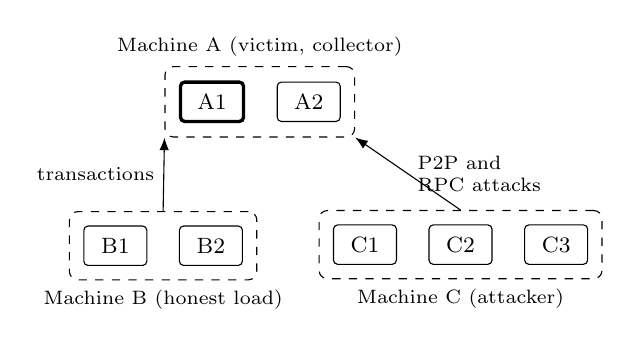
\begin{tikzpicture}[font=\footnotesize, node distance=4mm,
  n/.style={draw, rounded corners=1.5pt, minimum width=8mm, minimum height=5mm, inner sep=1.5pt},
  m/.style={draw, dashed, rounded corners=3pt, inner sep=5pt}]
\node[n, very thick] (a1) {A1};
\node[n, right=of a1] (a2) {A2};
\node[m, fit=(a1)(a2), label={[font=\scriptsize]above:Machine A (victim, collector)}] (ma) {};
\node[n, below left=13mm and 4mm of a1] (b1) {B1};
\node[n, right=of b1] (b2) {B2};
\node[m, fit=(b1)(b2), label={[font=\scriptsize]below:Machine B (honest load)}] (mb) {};
\node[n, below right=13mm and -1mm of a2] (c1) {C1};
\node[n, right=of c1] (c2) {C2};
\node[n, right=of c2] (c3) {C3};
\node[m, fit=(c1)(c3), label={[font=\scriptsize]below:Machine C (attacker)}] (mc) {};
\draw[-{Latex[length=1.6mm]}] (mb.north) -- node[left, font=\scriptsize]{transactions} (ma.south west);
\draw[-{Latex[length=1.6mm]}] (mc.north) -- node[right, font=\scriptsize, align=left]{P2P and\\RPC attacks} (ma.south east);
\end{tikzpicture}
\caption{Testbed. A1 is the single Clique sealer and the measurement point; all machines share an isolated WiFi LAN.}\label{fig:topology}
\end{figure}

\begin{table}[t]
\caption{Node Roles}\label{tab:nodes}
\centering\footnotesize
\setlength{\tabcolsep}{3pt}
\begin{tabular}{@{}lL{1.55cm}L{2.2cm}L{2.75cm}@{}}
\toprule
Mach. & Node(s) & Role & Scenarios \\
\midrule
A & A1 & Sealer, victim, collector & Target of all attacks \\
A & A2 & Honest peer & Benign reference \\
B & B1, B2 & Honest nodes & Background load, Flooding \\
C & C1--C3, spawned nodes & Attacker nodes & Sybil, Eclipse, RPC Abuse \\
\bottomrule
\end{tabular}
\end{table}

\subsection{Telemetry Collector}
A collector on Machine~A polls the local Geth instance and the operating system at a nominal interval of two seconds. Each cycle issues JSON-RPC calls (\code{net\_peerCount}, \code{admin\_peers}, \code{txpool\_status}, \code{eth\_getBlockByNumber}, and a timed \code{eth\_blockNumber} probe) and reads host counters through \code{psutil}. Table~\ref{tab:metrics} lists the 16 raw metrics. The collector also stores seven quantities derived from consecutive polls (first differences of peer count, block time, pending transactions, invalid transactions and gas used, and 30-second rates of pending transactions and peer churn), the timestamp, and the label, for 26 columns per record.

\begin{table}[t]
\caption{Raw Metrics and Telemetry Layers}\label{tab:metrics}
\centering\footnotesize
\begin{tabular}{@{}lL{3.9cm}l@{}}
\toprule
Layer & Metric & Source \\
\midrule
P2P & \code{peer\_count}, \code{subnet\_diversity}, \code{peer\_churn}, \code{p2p\_ingress\_rate} & Geth RPC \\
Chain & \code{gas\_used\_last\_block}, \code{pending\_tx\_count} & Geth RPC \\
RPC & \code{rpc\_latency\_ms} & Timed probe \\
Host & \code{cpu\_percent}, \code{ram\_percent} & OS \\
OS-network & \code{net\_bytes\_recv\_rate}, \code{net\_bytes\_sent\_rate}, \code{net\_connections} & OS \\
\midrule
Excluded & \code{block\_number}, \code{block\_time}, \code{blocks\_behind}, \code{tx\_invalid\_total} & Geth RPC \\
\bottomrule
\end{tabular}
\end{table}

\section{The HAIDS-PoA Dataset}\label{sec:dataset}
\subsection{Attack Scenarios}
One scenario is active per session, so labels are assigned at session level without conflict resolution. The adversary controls the nodes on Machine~C and has LAN access to the P2P and RPC interfaces of A1; it holds no sealer key and cannot modify the Geth binary.

\emph{Eclipse}~\cite{heilman2015,marcus2018,henningsen2019}. The attacker progressively removes honest peers from A1's peer table and inserts the three attacker nodes C1--C3, in cycles separated by 10--20~s, while honest nodes keep trying to reconnect. Isolation therefore succeeds and fails over time. Two 60-minute sessions were recorded.

\emph{Sybil}~\cite{douceur2002}. Machine~C runs the base nodes C1--C3 and five additional Geth identities that are repeatedly connected to and disconnected from A1, inflating and churning the peer table, together with request load from the attacker host. One 120-minute session was recorded.

\emph{Transaction Flooding}~\cite{baqer2016,pacheco2023}. The honest nodes B1 and B2 switch from their background rate of about 100 transactions per minute to multi-threaded submission at 3{,}000--6{,}000 transactions per minute, with elevated gas price to ensure mempool retention. Six sessions on two days were recorded.

\emph{RPC Abuse}~\cite{saad2020}. A script on Machine~C runs 230 concurrent threads that continuously submit computationally expensive JSON-RPC calls (\code{eth\_getLogs} over a large block range, \code{eth\_call} with an oversized payload, \code{eth\_getStorageAt}) to A1. Eighteen sessions on two days were recorded; several are short because the collector's own RPC calls time out under load.

\emph{Normal}. A1 seals blocks while honest nodes submit background transactions and periodic contract deployments. Eight sessions on three days were recorded. \tbc{which nodes ran the background transaction generator.}

Labels are encoded as 0~=~Normal, 1~=~Eclipse, 2~=~Flooding, 3~=~Sybil, 4~=~RPC Abuse. Records at the onset of an attack session carry the attack label although the attack may not yet have reached its steady state.

\subsection{Sessions and Class Distribution}
A recording session is a maximal run of records of one class without a gap longer than 60~s and without a reset of the block height. Table~\ref{tab:classes} gives the resulting structure. The dataset spans six calendar days between 8 and 16~April~2026. Normal operation is interleaved with Flooding on 11~April and with RPC Abuse on 13 and 16~April.

\begin{table}[t]
\caption{Class Distribution and Recording Structure}\label{tab:classes}
\centering\footnotesize
\setlength{\tabcolsep}{3.2pt}
\begin{tabular}{@{}lrrrrrrr@{}}
\toprule
Class & Records & \% & Sess. & Days & Hours & Block (s) & Poll (s) \\
\midrule
Normal & 15{,}301 & 51.9 & 8 & 3 & 8.88 & 15 & 2.0 \\
Eclipse & 3{,}416 & 11.6 & 2 & 2 & 2.00 & 5 & 2.0 \\
Flooding & 3{,}531 & 12.0 & 6 & 2 & 2.06 & 15 & 2.0 \\
Sybil & 3{,}541 & 12.0 & 1 & 1 & 2.00 & 5 & 2.0 \\
RPC Abuse & 3{,}683 & 12.5 & 18 & 2 & 3.68 & 15 & 3.0 \\
\midrule
Total & 29{,}472 & 100 & 35 & 6 & 18.62 & & \\
\bottomrule
\end{tabular}
\vspace{2pt}

{\raggedright\scriptsize Block: Clique block period observed in the session. Poll: median interval between consecutive records.\par}
\end{table}

\subsection{Recording Conditions That Differ Between Classes}\label{sec:conditions}
Three recording conditions are not constant across classes. They are visible in the data and are reported here because they constrain what a model may legitimately use.

\emph{Block period.} The sessions of 8--9~April (Eclipse and Sybil) ran with a 5-second block period; the chain was then re-initialised and all later sessions (Normal, Flooding, RPC Abuse) ran with 15~seconds. The block period, the block height and the inter-block time therefore identify the chain instance and are excluded from the model inputs. Quantities that depend on block production (\code{gas\_used\_last\_block} and, to a lesser degree, \code{pending\_tx\_count}) remain partly confounded with the block period for Eclipse and Sybil.

\emph{Sybil session.} Sybil was recorded in a single session, with millisecond-resolution timestamps and a median probe latency of 2~ms, against 33--74~ms in every Normal, Eclipse and Flooding session. This points to a different collector configuration for that session. \tbc{collector location and version used on 9~April.} Sybil results cannot be validated on an unseen day and should be read as an upper bound.

\emph{Polling interval.} Under RPC Abuse the collector's own calls are delayed and the median interval rises to 3~s. The interval is a consequence of the attack, but it also separates the Sybil session (2.03~s) from the others (2.00~s), so it is not used as a feature.

Two columns, \code{blocks\_behind} and \code{tx\_invalid\_total}, are constant (zero) in all 29{,}472 records and are excluded. No record contains missing values and no two records are identical.

\section{Methodology}\label{sec:method}
\subsection{Leakage-Free Preprocessing}\label{sec:preproc}
The pipeline follows four rules.
\begin{enumerate}
\item Records are never shuffled before feature engineering.
\item Every derived feature is causal (it uses the current and past records only) and is computed inside one recording session.
\item The class label is never used to build a feature.
\item Identifiers of the chain instance and of the collector (Section~\ref{sec:conditions}) are not model inputs.
\end{enumerate}
Twelve raw metrics are retained and grouped into five telemetry layers (Table~\ref{tab:metrics}). Seven heavy-tailed metrics (the three OS-network counters, \code{p2p\_ingress\_rate}, \code{gas\_used\_last\_block}, \code{pending\_tx\_count}, \code{rpc\_latency\_ms}) are transformed with $\log(1+x)$. For each metric $x$ and record $t$ of a session we add the rolling mean and standard deviation over a window of $W=5$ records (10~s at the nominal interval) and the first difference:
\begin{align}
\mu_t &= \tfrac{1}{n_t}\textstyle\sum_{i=t-n_t+1}^{t} x_i, \qquad n_t=\min(W,t),\\
\sigma_t &= \bigl(\tfrac{1}{n_t}\textstyle\sum_{i=t-n_t+1}^{t}(x_i-\mu_t)^2\bigr)^{1/2},\qquad \Delta_t = x_t-x_{t-1},
\end{align}
with $\Delta_1=0$. One additional feature, the logarithmic ratio of sent to received bytes, belongs to the OS-network layer. The result is 49 features: 8 for Host, 13 for OS-network, 16 for P2P, 8 for Chain and 4 for RPC. Standardisation, where a model requires it, is fitted on the training partition only. No feature selection is performed on the data; feature sets are defined a priori by telemetry layer, and their effect is studied by ablation.

\subsection{Evaluation Protocols}\label{sec:protocols}
We evaluate under three protocols of increasing strictness.

\emph{Random.} Records are shuffled and split 80/20, stratified by class. Rolling features of neighbouring records overlap, and neighbours fall on both sides of the split. This protocol is included because it is common practice, not because it is valid.

\emph{Within-session.} Each session is split chronologically: the first 80\% of its records are used for training and the last 20\% for testing, with a purge gap of $W$ records at the boundary so that no rolling window spans both sides. Sessions shorter than 50 records are used for training only. Training and test data come from the same sessions.

\emph{Cross-day.} Each class is divided into two sides, A and B, that share no recording day (Table~\ref{tab:folds}). Models are trained on one side and tested on the other, in both directions. Sybil has a single session; its two chronological halves are used, separated by a purge gap, and its results are flagged accordingly.

\begin{table}[t]
\caption{Cross-Day Protocol: Days and Records per Side}\label{tab:folds}
\centering\footnotesize
\begin{tabular}{@{}lllrr@{}}
\toprule
Class & Side A & Side B & A & B \\
\midrule
Normal & 11 Apr & 13, 16 Apr & 6{,}402 & 8{,}899 \\
Eclipse & 8 Apr & 9 Apr & 1{,}717 & 1{,}699 \\
Flooding & 10 Apr & 11 Apr & 860 & 2{,}671 \\
RPC Abuse & 13 Apr & 16 Apr & 2{,}908 & 775 \\
Sybil$^{\dagger}$ & first half & second half & 1{,}741 & 1{,}741 \\
\bottomrule
\end{tabular}
\vspace{2pt}

{\raggedright\scriptsize $^{\dagger}$Single session on 9~April; 59 records around the cut are discarded.\par}
\end{table}

All stochastic experiments are repeated with five seeds (0--4). We report the mean and the standard deviation over seeds and, for the cross-day protocol, over the two directions. Macro-averaged F1 over the five classes is the primary metric; accuracy, macro precision and recall, per-class recall and confusion matrices are also given.

\subsection{Models and Rationale}\label{sec:models}
The feature vectors are tabular, low-dimensional (49 features), heterogeneous in scale, and moderately sized ($\approx$29{,}000 records). The model set is chosen for this regime and for the two questions a node operator faces: which attack is in progress when attack labels exist, and whether anything abnormal is happening when they do not.

\emph{Logistic regression} is the linear reference. It shows how much of the task is linearly separable and whether more complex models are necessary.

\emph{Random Forest}~\cite{breiman2001}, \emph{XGBoost}~\cite{chen2016} and \emph{LightGBM}~\cite{ke2017} are tree ensembles, which remain the strongest family on medium-sized tabular data~\cite{grinsztajn2022}. They are invariant to monotone feature scaling, handle heavy-tailed counters without tuning, and have inference costs compatible with a two-second polling loop. The three differ in how trees are built (bagging of deep trees, level-wise boosting, leaf-wise boosting on histograms), which tests whether conclusions depend on a particular ensemble.

\emph{Isolation Forest}~\cite{liu2008} and a dense \emph{autoencoder}~\cite{sakurada2014} are trained on benign records only. They represent the situation in which labeled attack data are unavailable or the attack is new. Isolation Forest is a cheap partition-based baseline; the autoencoder learns the joint structure of benign telemetry and scores a record by its reconstruction error.

A recurrent sequence model is not included. The rolling statistics already encode the 10-second context that the two-second polling interval makes available, and the session structure leaves too few independent sequences per class (one to eighteen) to train and validate a sequence model without the session leakage this paper sets out to avoid.

For the benign-only detectors, the chronological last 15\% of every benign training session is held out as validation data. It serves two purposes: early stopping of the autoencoder, and threshold selection. The alarm threshold of each detector is the 99th percentile of its scores on this benign validation data, so no attack label and no test record is used to set it.

\subsection{Hyperparameters and Environment}
Hyperparameters were fixed before the experiments and were not tuned on test data (Table~\ref{tab:hp}). Class imbalance is handled with class weights inversely proportional to class frequency (balanced sample weights for XGBoost). All experiments ran on a single machine without GPU: Intel Xeon 2.10~GHz, 2~logical cores, 7.8~GB RAM, Linux, Python~3.10.20, scikit-learn~1.4.2, XGBoost~3.2.0, LightGBM~4.7.0, PyTorch~2.2.2, NumPy~1.26.4, pandas~2.1.4.

\begin{table}[t]
\caption{Hyperparameters (Seeds 0--4 for Every Model)}\label{tab:hp}
\centering\footnotesize
\begin{tabular}{@{}L{1.75cm}L{6.45cm}@{}}
\toprule
Model & Configuration \\
\midrule
Logistic regression & L2 penalty, $C=1$, L-BFGS solver, at most 2{,}000 iterations, balanced class weights, standardised inputs \\
Random Forest & 300 trees, maximum depth 15, minimum 20 samples per leaf and 40 per split, $\sqrt{d}$ features per split, Gini criterion, bootstrap, balanced class weights \\
XGBoost & 300 boosting rounds, maximum depth 4, learning rate 0.05, minimum child weight 30, row subsampling 0.7, column subsampling 0.7, $\alpha=1$, $\lambda=3$, $\gamma=0.5$, histogram tree method, multiclass log-loss, balanced sample weights \\
LightGBM & 200 boosting rounds, maximum depth 4, 15 leaves, learning rate 0.05, minimum 50 samples per leaf, row subsampling 0.7 every iteration, column subsampling 0.7, $\alpha=1$, $\lambda=2$, balanced class weights \\
Isolation Forest & 200 trees, 256 samples per tree, all features, fitted on benign records, standardised inputs \\
Autoencoder & Dense 49--64--32--8--32--64--49, ReLU, dropout 0.1 in the encoder, mean-squared-error loss, Adam optimiser, learning rate $10^{-3}$ (constant, no scheduler), weight decay $10^{-5}$, batch size 256, at most 200 epochs, early stopping with patience 15 on benign validation loss, standardised inputs clipped to $\pm 10$; 11{,}129 parameters \\
Thresholds & 99th percentile of benign validation scores (benign-only detectors); 0.5 on the predicted probability (supervised binary detector) \\
\bottomrule
\end{tabular}
\end{table}

No early stopping or learning-rate schedule is used for the boosted models: the number of rounds is fixed. The autoencoder stopped after a median of 163 epochs (range 116--200) across all runs.

\section{Results}\label{sec:results}
\subsection{Effect of the Evaluation Protocol}\label{sec:res-protocol}
Table~\ref{tab:protocol} and Fig.~\ref{fig:protocol} give the five-class results. Under the random and the within-session protocols every model, including logistic regression, is essentially perfect. On unseen days the macro-F1 falls to 0.80--0.87 and accuracy to 0.79--0.83. The data are identical in the three cases; only the relation between training and test records changes.

\begin{table}[t]
\caption{Five-Class Results Under Three Protocols (All 49 Features, Mean Over Five Seeds; Cross-Day Also Over Two Directions)}\label{tab:protocol}
\centering\footnotesize
\setlength{\tabcolsep}{3.5pt}
\begin{tabular}{@{}llccccc@{}}
\toprule
Protocol & Model & Acc. & Prec. & Rec. & Macro-F1 & $\pm$ \\
\midrule
\multirow{4}{*}{Random} & Logistic regr. & 1.000 & 1.000 & 1.000 & 1.000 & 0.000 \\
 & Random Forest & 1.000 & 1.000 & 1.000 & 1.000 & 0.000 \\
 & XGBoost & 1.000 & 0.999 & 1.000 & 1.000 & 0.001 \\
 & LightGBM & 1.000 & 1.000 & 1.000 & 1.000 & 0.000 \\
\midrule
\multirow{4}{*}{Within-session} & Logistic regr. & 0.999 & 0.999 & 1.000 & 0.999 & 0.000 \\
 & Random Forest & 1.000 & 1.000 & 1.000 & 1.000 & 0.000 \\
 & XGBoost & 1.000 & 1.000 & 1.000 & 1.000 & 0.000 \\
 & LightGBM & 1.000 & 1.000 & 1.000 & 1.000 & 0.000 \\
\midrule
\multirow{4}{*}{Cross-day} & Logistic regr. & 0.808 & 0.891 & 0.917 & 0.866 & 0.102 \\
 & Random Forest & 0.793 & 0.865 & 0.853 & 0.800 & 0.021 \\
 & XGBoost & 0.831 & 0.879 & 0.868 & 0.833 & 0.064 \\
 & LightGBM & 0.814 & 0.871 & 0.875 & 0.827 & 0.037 \\
\bottomrule
\end{tabular}
\end{table}

\begin{figure}[t]
\centering
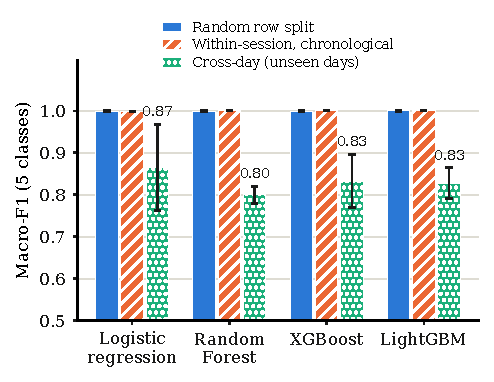
\includegraphics[width=0.95\columnwidth]{protocol_effect.pdf}
\caption{Macro-F1 of four classifiers under three evaluation protocols. Error bars: standard deviation over seeds and directions.}\label{fig:protocol}
\end{figure}

Table~\ref{tab:folddetail} separates the two cross-day directions. The standard deviations in Table~\ref{tab:protocol} mostly reflect the difference between directions, not between seeds: for a given direction the seed-to-seed standard deviation is at most 0.031. The errors are concentrated in two confusions (Fig.~\ref{fig:confusion}, left). Trained on side~A, the models label about half of the benign records of side~B (13 and 16~April) as Eclipse; trained on side~B, the three tree ensembles miss between 40\% and 77\% of the Eclipse records of 8~April, while logistic regression misses none. With LightGBM, Flooding and Sybil are recognised with recall of at least 0.94 in both directions, and RPC Abuse with 0.87 and 0.98. The ranking of models also changes with the protocol: logistic regression is the weakest model within sessions and has the highest average on unseen days, although with the largest spread.

\begin{table}[t]
\caption{Cross-Day Macro-F1 by Direction (Mean $\pm$ Std.\ Over Five Seeds)}\label{tab:folddetail}
\centering\footnotesize
\begin{tabular}{@{}lcc@{}}
\toprule
Model & Train A, test B & Train B, test A \\
\midrule
Logistic regression & $0.769 \pm 0.000$ & $0.962 \pm 0.000$ \\
Random Forest & $0.803 \pm 0.003$ & $0.796 \pm 0.031$ \\
XGBoost & $0.772 \pm 0.006$ & $0.893 \pm 0.008$ \\
LightGBM & $0.796 \pm 0.011$ & $0.859 \pm 0.023$ \\
\bottomrule
\end{tabular}
\end{table}

\begin{figure}[t]
\centering
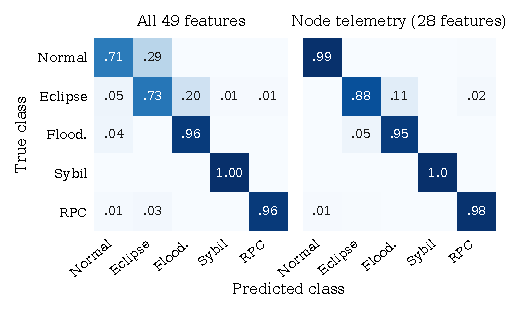
\includegraphics[width=\columnwidth]{confusion_cross_day.pdf}
\caption{Row-normalised cross-day confusion matrices of LightGBM, pooled over directions and seeds. Left: all features. Right: node telemetry only.}\label{fig:confusion}
\end{figure}

\subsection{Feature-Layer Ablation}\label{sec:res-ablation}
To identify which telemetry carries the attack and which carries the session, we retrain LightGBM while removing one layer at a time, and with one layer alone (Table~\ref{tab:ablation}, Fig.~\ref{fig:ablation}).

\begin{table*}[t]
\caption{Feature-Layer Ablation (LightGBM, Macro-F1, Five Seeds)}\label{tab:ablation}
\centering\footnotesize
\begin{tabular}{@{}L{5.6cm}rccl@{}}
\toprule
Feature set & $d$ & Within-session & Cross-day & Cross-day recall N / E / F / S / R \\
\midrule
All layers & 49 & 1.000 & $0.827 \pm 0.037$ & .75 / .73 / .97 / 1.0 / .93 \\
\midrule
without Host & 41 & 1.000 & $0.809 \pm 0.035$ & .71 / .70 / .97 / 1.0 / .93 \\
without OS-network & 36 & 1.000 & $\mathbf{0.981 \pm 0.008}$ & .98 / 1.0 / .97 / .98 / .98 \\
without P2P & 33 & 1.000 & $0.850 \pm 0.068$ & .74 / .82 / .97 / 1.0 / .90 \\
without Chain & 41 & 1.000 & $0.718 \pm 0.032$ & .66 / .50 / .97 / .99 / .93 \\
without RPC & 45 & 1.000 & $0.798 \pm 0.038$ & .72 / .73 / .97 / .98 / .83 \\
\midrule
Host only & 8 & 0.919 & $0.504 \pm 0.024$ & .52 / .37 / .62 / .59 / .70 \\
OS-network only & 13 & 0.977 & $0.496 \pm 0.042$ & .62 / .50 / .78 / .95 / .00 \\
P2P only & 16 & 0.944 & $0.896 \pm 0.004$ & .93 / .92 / .97 / .99 / .75 \\
Chain only & 8 & 0.892 & $0.893 \pm 0.003$ & .94 / .84 / .97 / .93 / .88 \\
RPC only & 4 & 0.835 & $0.761 \pm 0.049$ & .79 / .54 / .60 / 1.0 / .94 \\
\midrule
OS telemetry (Host + OS-network) & 21 & 0.996 & $0.657 \pm 0.079$ & .67 / .50 / .92 / .95 / .61 \\
Node telemetry (P2P + Chain + RPC) & 28 & 0.998 & $0.951 \pm 0.016$ & .99 / .88 / .97 / 1.0 / .98 \\
P2P + RPC & 20 & 0.993 & $0.961 \pm 0.005$ & .98 / .92 / .97 / 1.0 / .98 \\
\midrule
Point-in-time values only & 13 & 1.000 & $0.815 \pm 0.022$ & .74 / .73 / .97 / 1.0 / .88 \\
Rolling and delta only & 36 & 1.000 & $0.869 \pm 0.043$ & .80 / .83 / .97 / 1.0 / .96 \\
\bottomrule
\end{tabular}
\vspace{2pt}

{\centering\scriptsize N: Normal, E: Eclipse, F: Flooding, S: Sybil (same session), R: RPC Abuse.\par}
\end{table*}

\begin{figure}[t]
\centering
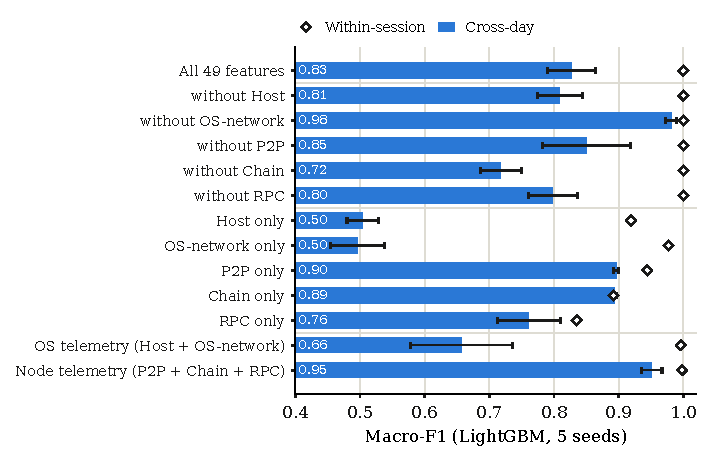
\includegraphics[width=\columnwidth]{ablation_layers.pdf}
\caption{Feature-layer ablation. Bars: cross-day macro-F1. Diamonds: within-session macro-F1 of the same feature set.}\label{fig:ablation}
\end{figure}

Three observations follow.

\emph{Within a session every layer looks useful.} Every feature set that combines at least two layers exceeds 0.97, and OS-network features alone reach 0.977. A within-session evaluation cannot distinguish attack signal from session signal.

\emph{Across days the layers separate.} OS-network features alone fall from 0.977 to 0.496, and they detect no RPC Abuse record on an unseen day. Host features alone fall from 0.919 to 0.504. P2P and Chain features alone lose little or nothing (0.944 to 0.896, 0.892 to 0.893). Node telemetry reaches 0.951 on unseen days and OS telemetry 0.657.

\emph{OS-network features are harmful, not merely uninformative.} Removing them raises the cross-day macro-F1 of the full model from 0.827 to 0.981 and removes the Normal--Eclipse confusion (Fig.~\ref{fig:confusion}, right, shows the same effect for node telemetry). The mechanism is visible in the raw data. The median number of open connections on Machine~A is 3{,}217 during Eclipse and 398 during benign operation overall, but benign sessions on 16~April have medians of 1{,}932 and 3{,}407. A model trained on 11~April learns that a high connection count means Eclipse, and a benign day with many open connections is then classified as an attack. The connection count describes the state of the host on a given day, not the state of the peer table. This is a shortcut in the sense of~\cite{geirhos2020}, and only the cross-day protocol exposes it.

Since the feature set ``without OS-network'' was identified on the test days, its score of 0.981 is an ablation result and not a tuned model. The node-telemetry set is defined a priori by where the measurement is taken, and we recommend it as the default input for this dataset. Within node telemetry, the Chain layer must be interpreted with care for Eclipse and Sybil because of the block-period difference (Section~\ref{sec:conditions}); the P2P and RPC layers together, which do not depend on block production, reach 0.961.

Rolling statistics help under shift: rolling and delta features alone outperform point-in-time values alone (0.869 against 0.815) although both are perfect within sessions.

\subsection{Benign-Only Detection and Unseen Attacks}\label{sec:res-anomaly}
Table~\ref{tab:anomaly} reports binary detection (attack against benign) on unseen days. The supervised detector is a LightGBM model trained on all attack classes and is the reference when labeled attacks are available.

\begin{table}[t]
\caption{Binary Detection on Unseen Days (All 49 Features, Five Seeds, Two Directions). Thresholds of Benign-Only Detectors Are Label-Free}\label{tab:anomaly}
\centering\footnotesize
\setlength{\tabcolsep}{3pt}
\begin{tabular}{@{}L{2.35cm}cccccc@{}}
\toprule
Detector & AUC & F1 & $\pm$ & Prec. & Rec. & FPR \\
\midrule
Isolation Forest & 0.988 & 0.695 & 0.278 & 0.970 & 0.625 & 0.035 \\
Autoencoder & 0.995 & 0.969 & 0.008 & 0.966 & 0.973 & 0.040 \\
IF \textsc{or} AE & 0.997 & 0.965 & 0.010 & 0.959 & 0.974 & 0.049 \\
IF \textsc{and} AE & 0.991 & 0.699 & 0.282 & 0.978 & 0.625 & 0.025 \\
\midrule
LightGBM (supervised, all attacks seen) & 0.993 & 0.990 & 0.005 & 0.995 & 0.985 & 0.005 \\
\bottomrule
\end{tabular}
\end{table}

\emph{Binary detection transfers across days.} The supervised binary detector keeps an F1 of 0.990 on unseen days with the same 49 features for which the five-class model drops to 0.827. The union of four attack classes cannot be separated from benign operation by a single session fingerprint, so the model relies on features that reflect the attacks.

\emph{The autoencoder is close to the supervised reference without attack labels.} It reaches an F1 of 0.969 with a false-positive rate of 4.0\%, above the 1\% targeted by the threshold. Within sessions its false-positive rate is 4.3\%, so most of the excess is already present without day shift.

\emph{Scores transfer; thresholds do not.} Isolation Forest ranks records almost as well as the autoencoder (AUC 0.988) but its F1 is 0.955 in one direction and 0.435 in the other, where the benign-validation threshold lets only 28\% of the attack records through. The threshold of a benign-only detector must therefore be recalibrated on recent benign data of the deployment. Combining the two detectors does not help: the \textsc{or} rule equals the autoencoder and the \textsc{and} rule equals Isolation Forest.

\emph{Unseen attacks.} Table~\ref{tab:zeroday} removes one attack class from the training data of the supervised detector and measures its recall on that class on unseen days. The supervised detector detects 0.4\% of Flooding and 8.8\% of RPC Abuse records when it has never seen them, 30\% of Sybil and 49\% of Eclipse. The autoencoder, which never sees any attack, detects 88--100\%. This is the case for keeping a benign-only model in the pipeline even when a supervised classifier performs better on known attacks.

\begin{table}[t]
\caption{Recall on an Attack Class Absent From Supervised Training (Cross-Day, All Features, Five Seeds)}\label{tab:zeroday}
\centering\footnotesize
\begin{tabular}{@{}lccc@{}}
\toprule
Held-out attack & LightGBM (unseen) & Isolation Forest & Autoencoder \\
\midrule
Eclipse & 0.490 & 0.788 & 0.999 \\
Flooding & 0.004 & 0.499 & 0.969 \\
Sybil$^{\dagger}$ & 0.303 & 0.705 & 0.998 \\
RPC Abuse & 0.088 & 0.516 & 0.876 \\
\bottomrule
\end{tabular}
\vspace{2pt}

{\raggedright\scriptsize $^{\dagger}$Same-session halves.\par}
\end{table}

With node telemetry only, the autoencoder is less effective (F1 $0.872 \pm 0.131$, recall 0.66 on RPC Abuse), while the supervised detector is unchanged (0.996). Host load is a legitimate indicator of RPC Abuse and Flooding for a model that only knows benign behaviour, and removing it costs recall. The feature set that is best for naming attacks is thus not the best for benign-only detection, which is a further argument for separating the two stages.

\subsection{Detection-Pipeline Ablation}\label{sec:res-pipeline}
The reference deployment of HAIDS-PoA (Section~\ref{sec:deployment}) chains an anomaly stage, an attack-typing stage and a decision stage that votes over consecutive polls. Table~\ref{tab:pipeline} isolates the contribution of each choice under the cross-day protocol with all features.

\begin{table}[t]
\caption{Detection-Pipeline Ablation (Cross-Day, All Features, Five Seeds, Two Directions)}\label{tab:pipeline}
\centering\footnotesize
\setlength{\tabcolsep}{3.5pt}
\begin{tabular}{@{}L{3.6cm}ccc@{}}
\toprule
\multicolumn{4}{@{}l}{\emph{(a) Stage structure}}\\
Pipeline & A$\to$B & B$\to$A & Mean \\
\midrule
Single stage: 5-class LightGBM, macro-F1 & 0.796 & 0.859 & 0.827 \\
Two stages: autoencoder alarm, then LightGBM typing, macro-F1 & 0.938 & 0.846 & 0.892 \\
Binary F1, single stage & 0.744 & 0.983 & 0.864 \\
Binary F1, two stages & 0.970 & 0.968 & 0.969 \\
Typing accuracy given an alarm & 0.989 & 0.880 & 0.935 \\
\bottomrule
\end{tabular}

\vspace{5pt}
\begin{tabular}{@{}lccccc@{}}
\toprule
\multicolumn{6}{@{}l}{\emph{(b) Temporal vote of the decision stage (autoencoder alarms)}}\\
Vote & FPR & Recall & F1 & False alarms/h & Delay (s) \\
\midrule
1-of-1 (none) & 0.040 & 0.973 & 0.969 & 15.9 & 0.0 \\
2-of-3 & 0.037 & 0.973 & 0.970 & 7.5 & 2.5 \\
3-of-5 & 0.037 & 0.972 & 0.969 & 6.0 & 4.8 \\
5-of-5 & 0.019 & 0.949 & 0.965 & 4.9 & 10.3 \\
\bottomrule
\end{tabular}
\vspace{2pt}

{\raggedright\scriptsize False alarms/h: distinct alarm episodes per hour of benign operation. Delay: median time from the first record of an attack session to the first alarm.\par}
\end{table}

\emph{Two stages against one.} Letting the benign-only autoencoder decide whether there is an attack, and a classifier trained on attack records only decide which one, raises the macro-F1 from 0.827 to 0.892 and makes the binary decision stable across directions (0.970 and 0.968, against 0.744 and 0.983 for the single-stage model). The gain comes from the direction in which the single-stage classifier mistakes a benign day for Eclipse. In the other direction the two-stage pipeline is slightly worse (0.846 against 0.859) because the typing stage inherits the Eclipse confusion.

\emph{Temporal vote.} Requiring $k$ alarms among the last $n$ polls barely changes record-level metrics but changes what an operator sees. A 3-of-5 vote reduces the number of distinct false-alarm episodes from 15.9 to 6.0 per benign hour at the cost of a median detection delay of 4.8~s. Every attack session of at least 30 records is detected under all four settings; the longest delay to the first alarm is 312--320~s, for one RPC Abuse session.

\subsection{Computational Cost}\label{sec:res-cost}
Table~\ref{tab:complexity} gives the dominant terms of training and inference complexity and Table~\ref{tab:cost} the measurements. Notation: $N$ training records, $d$ features, $K$ classes, $T$ trees, $h$ tree depth, $R$ boosting rounds, $I$ solver iterations, $\psi$ subsample size, $E$ epochs, $P$ network parameters. For boosted trees the histogram method makes the cost of one round linear in $N d$ with a small constant after binning; for Random Forest the $\log N$ factor is bounded by the depth limit.

\begin{table}[t]
\caption{Dominant Complexity Terms}\label{tab:complexity}
\centering\footnotesize
\begin{tabular}{@{}lll@{}}
\toprule
Model & Training & Inference (per record) \\
\midrule
Logistic regression & $O(I\,N\,d\,K)$ & $O(d\,K)$ \\
Random Forest & $O(T\,\sqrt{d}\,N\log N)$ & $O(T\,h)$ \\
XGBoost, LightGBM & $O(R\,K\,N\,d)$ & $O(R\,K\,h)$ \\
Isolation Forest & $O(T\,\psi\log\psi)$ & $O(T\log\psi)$ \\
Autoencoder & $O(E\,N\,P)$ & $O(P)$ \\
\bottomrule
\end{tabular}
\end{table}

\begin{table}[t]
\caption{Measured Cost (Cross-Day Training Side A, $N=13{,}628$, $d=49$; Benign-Only Models $N=5{,}426$)}\label{tab:cost}
\centering\footnotesize
\setlength{\tabcolsep}{3.2pt}
\begin{tabular}{@{}lrrrrr@{}}
\toprule
 & Train & \multicolumn{2}{c}{Single record (ms)} & Batch & Size \\
Model & (s) & median & p95 & (rec./s) & (MB) \\
\midrule
Logistic regression & $0.05 \pm 0.00$ & 0.19 & 0.26 & 2{,}421{,}719 & $<$0.01 \\
Random Forest & $4.37 \pm 0.11$ & 7.24 & 10.09 & 77{,}467 & 1.17 \\
XGBoost & $1.27 \pm 0.59$ & 0.44 & 0.57 & 284{,}635 & 1.11 \\
LightGBM & $0.68 \pm 0.05$ & 0.67 & 0.98 & 155{,}914 & 0.53 \\
Isolation Forest & $0.31 \pm 0.04$ & 2.54 & 3.55 & 97{,}137 & 1.58 \\
Autoencoder & $5.82 \pm 0.92$ & 0.32 & 0.46 & 1{,}203{,}678 & 0.05 \\
\bottomrule
\end{tabular}
\vspace{2pt}

{\raggedright\scriptsize Train: mean $\pm$ std.\ over five fits. Single record: 50 warm-up calls, then 1{,}000 timed calls. Batch: 1{,}024 records, median of 20 calls. Timer around \code{fit} and \code{predict} only; CPU only (Intel Xeon 2.10~GHz, 2 logical cores). Random Forest and Isolation Forest predict on one thread. Autoencoder: 169 epochs on average, 0.035~s per epoch.\par}
\end{table}

All models train in under six seconds on two CPU cores and score a single record in under 8~ms, three orders of magnitude below the two-second polling interval. Building one feature vector from the last five polls takes 26~ms with the unoptimised reference implementation, which is more than any model's inference time. On this dataset, computational cost does not discriminate between models; robustness to day shift does.

\subsection{Observations From a Reference Deployment}\label{sec:deployment}
HAIDS-PoA was collected as part of a multi-agent intrusion detection prototype in which a Collector agent polls the node, an Analyzer agent scores each record, a Decision agent produces an explanation of each alert with a small language model (TinyLlama, 1.1~billion parameters, with a LoRA adapter, on CPU), and a Blockchain agent records alerts through a smart contract. The prototype is not evaluated in this paper, but two observations from its logs motivate the benchmark.

In a ten-minute run against the live testnet on 23~April~2026, a first-generation Analyzer flagged 278 of 279 polls as anomalous. Its detectors had been validated within sessions only and used chain-instance identifiers such as the block height among their inputs, and the run took place one week after the last recording session. No ground truth was logged for that run, so the alarm rate cannot be converted into a false-positive rate, but the behaviour is consistent with what Sections~\ref{sec:res-protocol} and~\ref{sec:res-ablation} predict for a model that has learned session identifiers.

In the same run, producing one explanation took a median of 61~s (range 52--64~s), against a polling interval of 2~s; 247 of 256 queued alerts were dropped by the bounded queue. Model inference is therefore not the bottleneck of such an architecture (Table~\ref{tab:cost}); the explanation stage is, and it must be decoupled from detection and applied to voted alarm episodes rather than to individual polls. An end-to-end evaluation of the multi-agent system on labeled live traffic is left to future work.

\section{Ethical Considerations}\label{sec:ethics}
All attacks were executed inside a private testnet on a WiFi LAN isolated from the Internet. No public blockchain node, real user funds or externally deployed contract was involved. The dataset contains no personal data: all accounts, keys and enode identifiers were generated for this research, and nodes are referred to by the labels A1, A2, B1, B2, C1--C3. The four attack classes are documented in the literature~\cite{heilman2015,marcus2018,douceur2002,baqer2016,saad2020}; the paper and the repository describe them at the level needed to interpret the telemetry and to reproduce the benchmark.

\section{Limitations and Threats to Validity}\label{sec:threats}
\emph{Session confounding is reduced, not eliminated.} Four of five classes were recorded on two or three days, which is the minimum for a cross-day test. Each side of the cross-day protocol contains one to three days per class, so day-to-day variability is estimated from few days, as the difference between the two directions shows.

\emph{Sybil.} Sybil has one session, recorded with a different collector configuration (Section~\ref{sec:conditions}). Its cross-day figures are within-session figures and its RPC-latency signature should not be interpreted.

\emph{Block period.} Eclipse and Sybil were recorded with a 5-second block period and the other classes with 15~seconds. Chain-layer features are partly confounded for these two classes. The P2P + RPC result (0.961) is free of this effect for Eclipse.

\emph{Single sealer.} With one validator, in-turn and out-of-turn sealing, validator rotation and fork resolution are absent. Attacks whose effect is to delay or reorder block production among validators~\cite{ekparinya2020} cannot be studied.

\emph{Network and platform.} All machines run Windows~11 on one indoor WiFi LAN. Absolute values of latency and throughput features will differ in wide-area consortia, and thresholds will need recalibration.

\emph{Labels.} Labels are assigned per session. Onset records carry the attack label before the attack reaches its steady state, and no record-level injection log exists.

\emph{Attack diversity.} Each attack is one implementation with one set of parameters. Low-rate or adaptive variants are not covered, and an adversary aware of the detector is outside the scope.

\emph{Hyperparameters.} Hyperparameters were fixed a priori and not tuned. Tuning under the within-session protocol would not change scores that are already at 1.00; tuning under the cross-day protocol would require a third set of days that the dataset does not contain.

\emph{Timing measurements} were taken on a server CPU, not on the testbed machines.

\section{Future Work}\label{sec:future}
The most valuable extension is additional recording days for every class, in particular Sybil, with benign operation interleaved on each day and a single block period, so that a leave-one-day-out protocol with a separate validation day becomes possible. A multi-validator Clique configuration would bring consensus-level attacks into scope. A record-level injection log would allow onset detection to be evaluated precisely. Finally, the multi-agent prototype should be evaluated end to end on labeled live traffic, including the latency of each stage and the usefulness of the generated explanations.

\section{Conclusion}\label{sec:conclusion}
HAIDS-PoA provides 29{,}472 labeled records of node-state telemetry from an Ethereum Clique PoA testbed, covering benign operation and four attacks, with recording sessions preserved. This structure allows detectors to be tested on days they have not seen, and the test changes the conclusions. Classifiers that are perfect within sessions lose 13 to 20 points of macro-F1 on unseen days. The loss is caused by operating-system telemetry that fingerprints the recording session: node-level telemetry reaches 0.95 where operating-system telemetry reaches 0.66. Deciding whether an attack is in progress transfers across days while naming the attack is fragile, which favours a two-stage pipeline. A supervised detector is nearly blind to attack types it was not trained on, whereas an autoencoder trained on benign data detects them, provided that its threshold is recalibrated. We release the data, the leakage-free pipeline and every result file so that these findings can be reproduced and so that future detectors for PoA networks are evaluated across recording sessions.

\bibliographystyle{IEEEtran}
\begin{thebibliography}{10}
\bibitem{zheng2018} Z.~Zheng, S.~Xie, H.-N.~Dai, X.~Chen, and H.~Wang, ``Blockchain challenges and opportunities: A survey,'' \emph{Int. J. Web Grid Serv.}, vol.~14, no.~4, pp.~352--375, 2018.
\bibitem{wood2014} G.~Wood, ``Ethereum: A secure decentralised generalised transaction ledger,'' Ethereum Project Yellow Paper, 2014.
\bibitem{deangelis2018} S.~De~Angelis, L.~Aniello, R.~Baldoni, F.~Lombardi, A.~Margheri, and V.~Sassone, ``PBFT vs proof-of-authority: Applying the CAP theorem to permissioned blockchain,'' in \emph{Proc. Italian Conf. Cyber Security (ITASEC)}, 2018.
\bibitem{eip225} P.~Szil\'agyi, ``EIP-225: Clique proof-of-authority consensus protocol,'' Ethereum Improvement Proposals, 2017. [Online]. Available: \url{https://eips.ethereum.org/EIPS/eip-225}
\bibitem{heilman2015} E.~Heilman, A.~Kendler, A.~Zohar, and S.~Goldberg, ``Eclipse attacks on Bitcoin's peer-to-peer network,'' in \emph{Proc. 24th USENIX Security Symp.}, 2015, pp.~129--144.
\bibitem{marcus2018} Y.~Marcus, E.~Heilman, and S.~Goldberg, ``Low-resource eclipse attacks on Ethereum's peer-to-peer network,'' IACR Cryptology ePrint Archive, Rep. 2018/236, 2018.
\bibitem{douceur2002} J.~R.~Douceur, ``The Sybil attack,'' in \emph{Proc. 1st Int. Workshop Peer-to-Peer Systems (IPTPS)}, 2002, pp.~251--260.
\bibitem{baqer2016} K.~Baqer, D.~Y.~Huang, D.~McCoy, and N.~Weaver, ``Stressing out: Bitcoin `stress testing','' in \emph{Financial Cryptography and Data Security Workshops}, 2016, pp.~3--18.
\bibitem{tavallaee2009} M.~Tavallaee, E.~Bagheri, W.~Lu, and A.~A.~Ghorbani, ``A detailed analysis of the KDD CUP 99 data set,'' in \emph{Proc. IEEE Symp. Computational Intelligence for Security and Defense Applications (CISDA)}, 2009, pp.~1--6.
\bibitem{sharafaldin2018} I.~Sharafaldin, A.~H.~Lashkari, and A.~A.~Ghorbani, ``Toward generating a new intrusion detection dataset and intrusion traffic characterization,'' in \emph{Proc. 4th Int. Conf. Information Systems Security and Privacy (ICISSP)}, 2018, pp.~108--116.
\bibitem{saad2020} M.~Saad, J.~Spaulding, L.~Njilla, C.~Kamhoua, S.~Shetty, D.~Nyang, and D.~Mohaisen, ``Exploring the attack surface of blockchain: A comprehensive survey,'' \emph{IEEE Commun. Surveys Tuts.}, vol.~22, no.~3, pp.~1977--2008, 2020.
\bibitem{sommer2010} R.~Sommer and V.~Paxson, ``Outside the closed world: On using machine learning for network intrusion detection,'' in \emph{Proc. IEEE Symp. Security and Privacy}, 2010, pp.~305--316.
\bibitem{arp2022} D.~Arp, E.~Quiring, F.~Pendlebury, A.~Warnecke, F.~Pierazzi, C.~Wressnegger, L.~Cavallaro, and K.~Rieck, ``Dos and don'ts of machine learning in computer security,'' in \emph{Proc. 31st USENIX Security Symp.}, 2022, pp.~3971--3988.
\bibitem{kapoor2023} S.~Kapoor and A.~Narayanan, ``Leakage and the reproducibility crisis in machine-learning-based science,'' \emph{Patterns}, vol.~4, no.~9, Art. no. 100804, 2023.
\bibitem{pendlebury2019} F.~Pendlebury, F.~Pierazzi, R.~Jordaney, J.~Kinder, and L.~Cavallaro, ``TESSERACT: Eliminating experimental bias in malware classification across space and time,'' in \emph{Proc. 28th USENIX Security Symp.}, 2019, pp.~729--746.
\bibitem{kdd99} ``KDD Cup 1999 data,'' UCI KDD Archive, 1999. [Online]. Available: \url{http://kdd.ics.uci.edu/databases/kddcup99/kddcup99.html}
\bibitem{moustafa2015} N.~Moustafa and J.~Slay, ``UNSW-NB15: A comprehensive data set for network intrusion detection systems,'' in \emph{Proc. Military Communications and Information Systems Conf. (MilCIS)}, 2015, pp.~1--6.
\bibitem{alsaedi2020} A.~Alsaedi, N.~Moustafa, Z.~Tari, A.~Mahmood, and A.~Anwar, ``TON\_IoT telemetry dataset: A new generation dataset of IoT and IIoT for data-driven intrusion detection systems,'' \emph{IEEE Access}, vol.~8, pp.~165130--165150, 2020.
\bibitem{cicids2018} Canadian Institute for Cybersecurity, ``CSE-CIC-IDS2018 on AWS,'' 2018. [Online]. Available: \url{https://www.unb.ca/cic/datasets/ids-2018.html}
\bibitem{buczak2016} A.~L.~Buczak and E.~Guven, ``A survey of data mining and machine learning methods for cyber security intrusion detection,'' \emph{IEEE Commun. Surveys Tuts.}, vol.~18, no.~2, pp.~1153--1176, 2016.
\bibitem{luu2016} L.~Luu, D.-H.~Chu, H.~Olickel, P.~Saxena, and A.~Hobor, ``Making smart contracts smarter,'' in \emph{Proc. ACM SIGSAC Conf. Computer and Communications Security (CCS)}, 2016, pp.~254--269.
\bibitem{bartoletti2020} M.~Bartoletti, S.~Carta, T.~Cimoli, and R.~Saia, ``Dissecting Ponzi schemes on Ethereum: Identification, analysis, and impact,'' \emph{Future Gener. Comput. Syst.}, vol.~102, pp.~259--277, 2020.
\bibitem{wu2022} J.~Wu, Q.~Yuan, D.~Lin, W.~You, W.~Chen, C.~Chen, and Z.~Zheng, ``Who are the phishers? Phishing scam detection on Ethereum via network embedding,'' \emph{IEEE Trans. Syst., Man, Cybern., Syst.}, vol.~52, no.~2, pp.~1156--1166, 2022.
\bibitem{henningsen2019} S.~Henningsen, D.~Teunis, M.~Florian, and B.~Scheuermann, ``Eclipsing Ethereum peers with false friends,'' in \emph{Proc. IEEE European Symp. Security and Privacy Workshops (EuroS\&PW)}, 2019.
\bibitem{platt2023} M.~Platt and P.~McBurney, ``Sybil in the haystack: A comprehensive review of blockchain consensus mechanisms in search of strong Sybil attack resistance,'' \emph{Algorithms}, vol.~16, no.~1, Art. no. 34, 2023.
\bibitem{ekparinya2020} P.~Ekparinya, V.~Gramoli, and G.~Jourjon, ``The attack of the clones against proof-of-authority,'' in \emph{Proc. Network and Distributed System Security Symp. (NDSS)}, 2020.
\bibitem{khoa2024} T.~V.~Khoa, D.~H.~Son, D.~T.~Hoang, N.~L.~Trung, T.~T.~T.~Quynh, D.~N.~Nguyen, N.~V.~Ha, and E.~Dutkiewicz, ``Real-time cyberattack detection with collaborative learning for blockchain networks,'' arXiv:2407.04011, 2024.
\bibitem{engelen2021} G.~Engelen, V.~Rimmer, and W.~Joosen, ``Troubleshooting an intrusion detection dataset: The CICIDS2017 case study,'' in \emph{Proc. IEEE Security and Privacy Workshops (SPW)}, 2021, pp.~7--12.
\bibitem{geirhos2020} R.~Geirhos, J.-H.~Jacobsen, C.~Michaelis, R.~Zemel, W.~Brendel, M.~Bethge, and F.~A.~Wichmann, ``Shortcut learning in deep neural networks,'' \emph{Nature Mach. Intell.}, vol.~2, no.~11, pp.~665--673, 2020.
\bibitem{pacheco2023} M.~Pacheco, G.~A.~Oliva, G.~K.~Rajbahadur, and A.~E.~Hassan, ``What makes Ethereum blockchain transactions be processed fast or slow? An empirical study,'' \emph{Empir. Softw. Eng.}, vol.~28, 2023, doi: 10.1007/s10664-022-10283-7.
\bibitem{breiman2001} L.~Breiman, ``Random forests,'' \emph{Mach. Learn.}, vol.~45, no.~1, pp.~5--32, 2001.
\bibitem{chen2016} T.~Chen and C.~Guestrin, ``XGBoost: A scalable tree boosting system,'' in \emph{Proc. 22nd ACM SIGKDD Int. Conf. Knowledge Discovery and Data Mining}, 2016, pp.~785--794.
\bibitem{ke2017} G.~Ke, Q.~Meng, T.~Finley, T.~Wang, W.~Chen, W.~Ma, Q.~Ye, and T.-Y.~Liu, ``LightGBM: A highly efficient gradient boosting decision tree,'' in \emph{Advances in Neural Information Processing Systems}, vol.~30, 2017.
\bibitem{grinsztajn2022} L.~Grinsztajn, E.~Oyallon, and G.~Varoquaux, ``Why do tree-based models still outperform deep learning on typical tabular data?'' in \emph{Advances in Neural Information Processing Systems}, vol.~35, 2022.
\bibitem{liu2008} F.~T.~Liu, K.~M.~Ting, and Z.-H.~Zhou, ``Isolation forest,'' in \emph{Proc. IEEE Int. Conf. Data Mining (ICDM)}, 2008, pp.~413--422.
\bibitem{sakurada2014} M.~Sakurada and T.~Yairi, ``Anomaly detection using autoencoders with nonlinear dimensionality reduction,'' in \emph{Proc. 2nd Workshop Machine Learning for Sensory Data Analysis (MLSDA)}, 2014, pp.~4--11.
\end{thebibliography}

\end{document}
